Cette annexe a pour raison d'être, de donner une précision sur les end-points de l'implémentation finale de notre \textit{API} de synthèse.
Pour l'\textit{end-point} \textbf{\textit{POST /extractive-gensim}}, voici un exemple de requête réussie :
\begin{center}
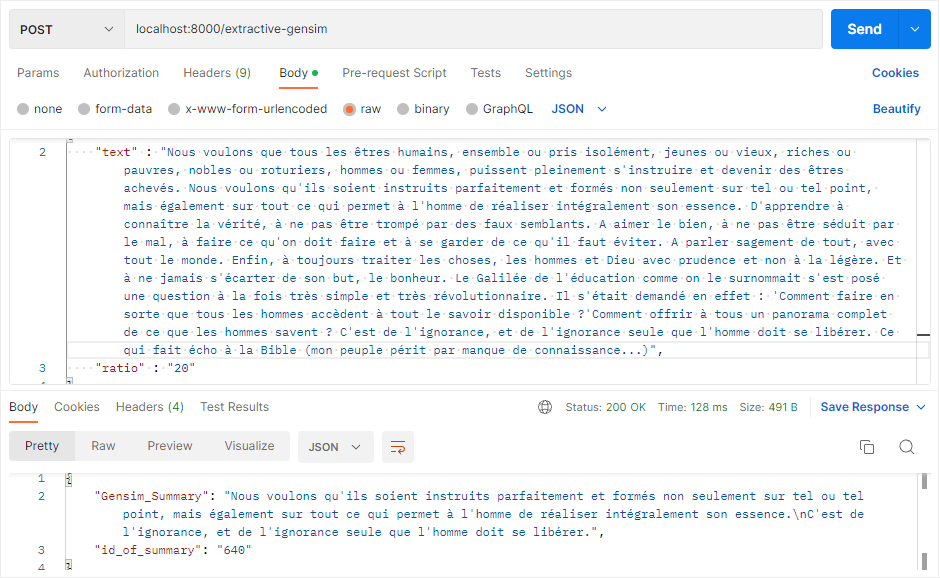
\includegraphics[width=15cm]{GensimText.PNG}
\end{center}
Mais pour la réussite de toute requête, il faudra préciser le paramètre \textit{\textbf{api-key}} dans les \textit{headers}. Ce paramètre aura pour valeur la clé générée à travers l'\textit{API} pour avoir les autorisations. Voici comment c'est précisé dans la requête précédente :
\begin{center}
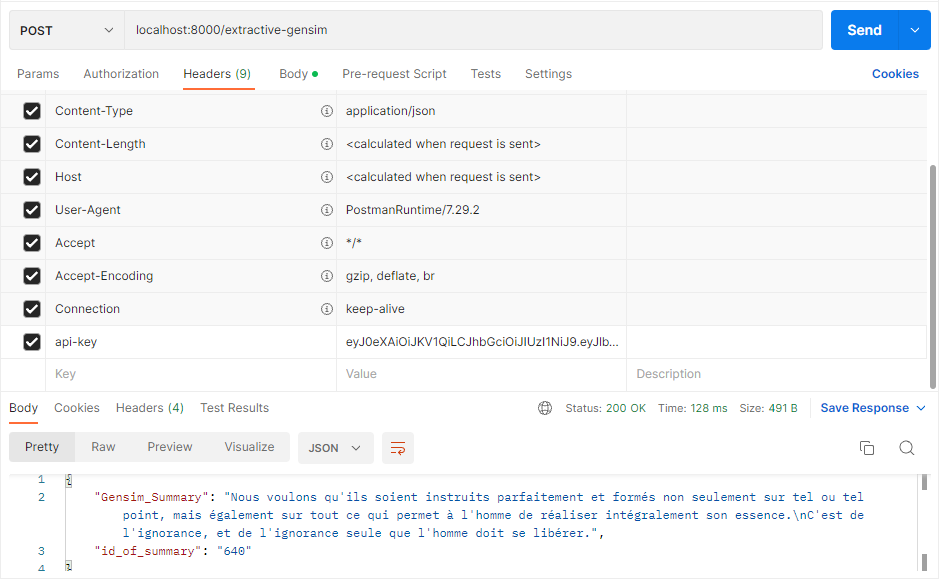
\includegraphics[width=15cm]{GensimAuth.PNG}
\end{center}
En cas d'erreur de clé, un exemple de message est le suivant :
\begin{center}
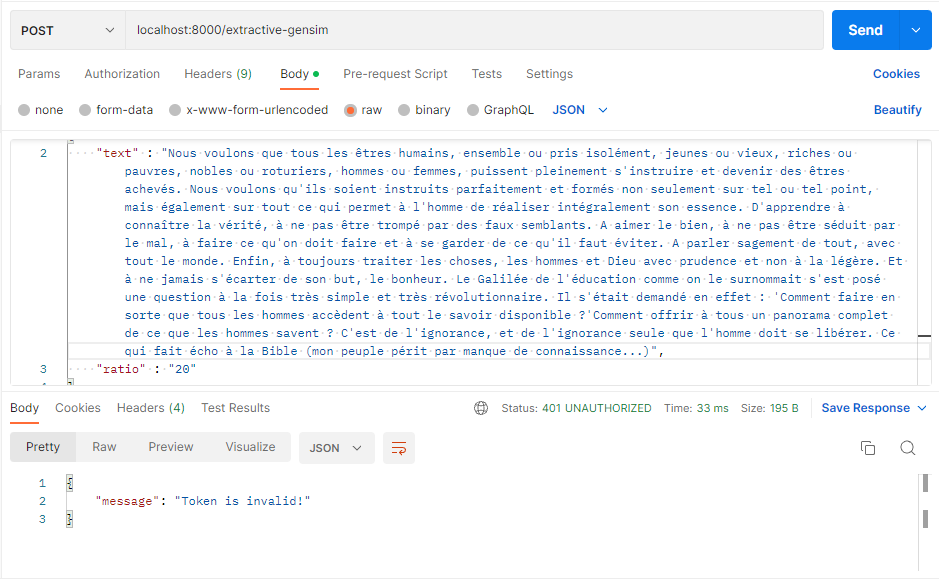
\includegraphics[width=15cm]{GensimInvalidKey.PNG}
\end{center}
Si on précise un \textit{ratio} inapproprié, le message, pour tous les cas, est le suivant :
\begin{center}
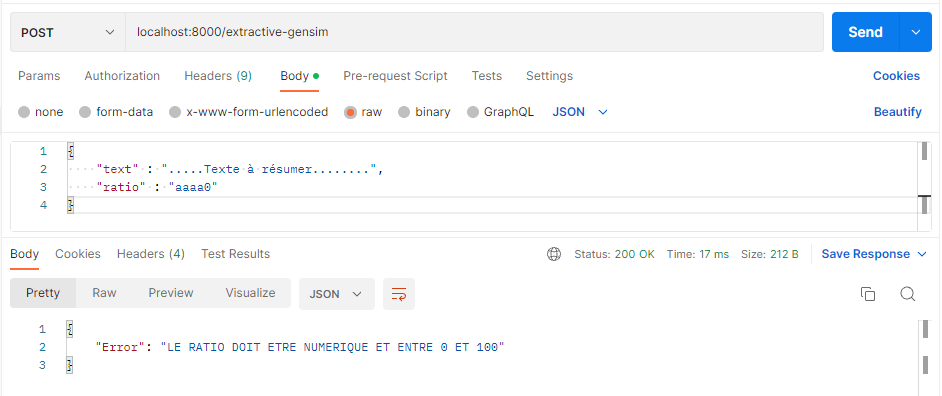
\includegraphics[width=15cm]{GensionRatioError.PNG}
\end{center}

Pour l'\textit{end-point} \textbf{\textit{POST /extractive-merge}}, voici un exemple de requête :
\begin{center}
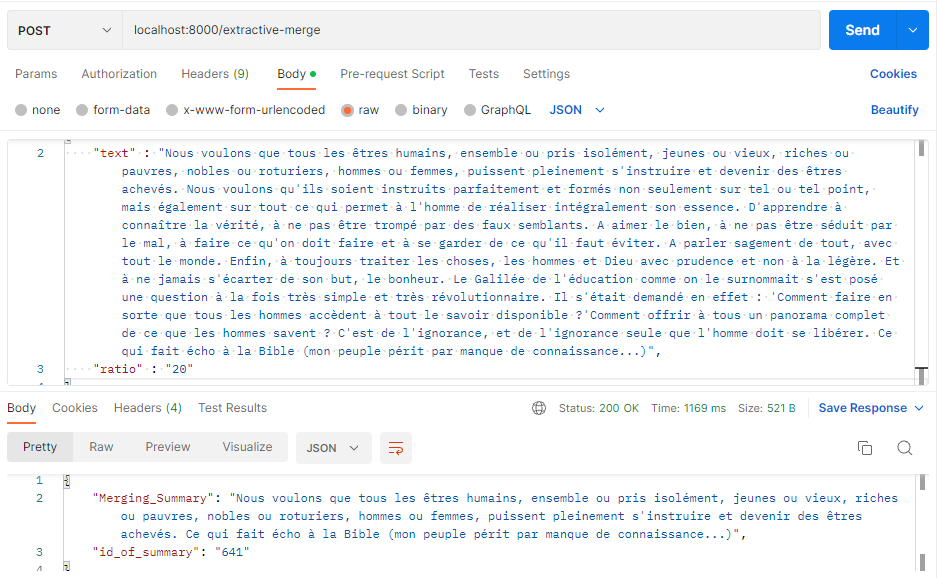
\includegraphics[width=15cm]{MergingText.PNG}
\end{center}

Pour la partie de synthèse abstractive en utilisant \textit{BART}, pour les petits documents, c'est-à-dire l'\textit{end-point} \textbf{\textit{POST /abstractive-large}}, voici un exemple de requête réussie :
\begin{center}
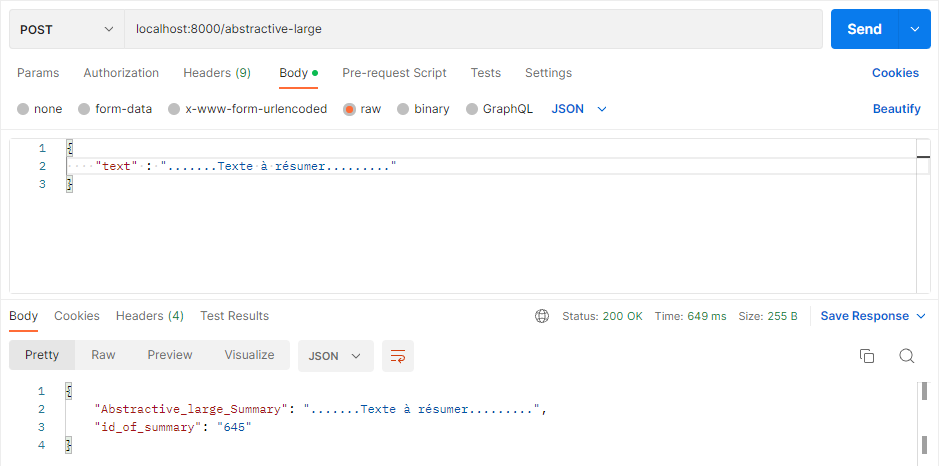
\includegraphics[width=15cm]{AbstractiveLarge.PNG}
\end{center}

Au cas où la taille est dépassée pour la partie petits documents, voici un exemple de requête :
\begin{center}
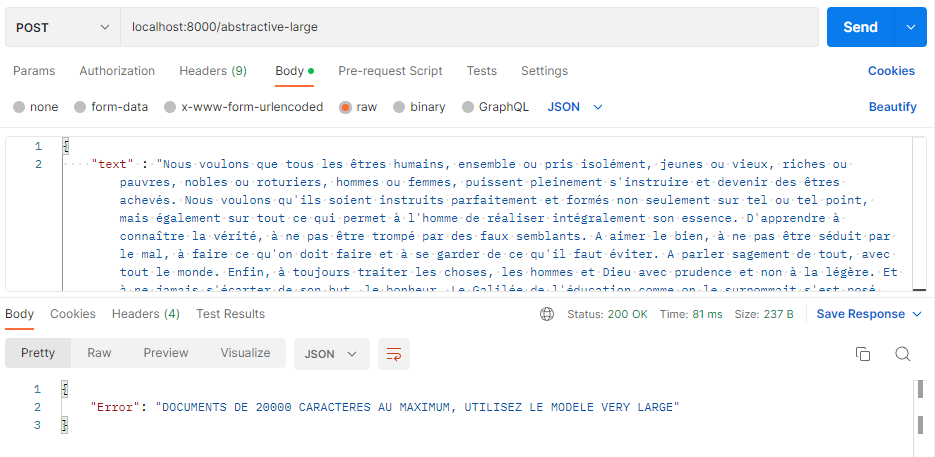
\includegraphics[width=15cm]{AbstractiveLargeError.PNG}
\end{center}

Pour l'\textit{end-point} \textbf{\textit{POST /abstractive-very-large}}, voici un exemple :
\begin{center}
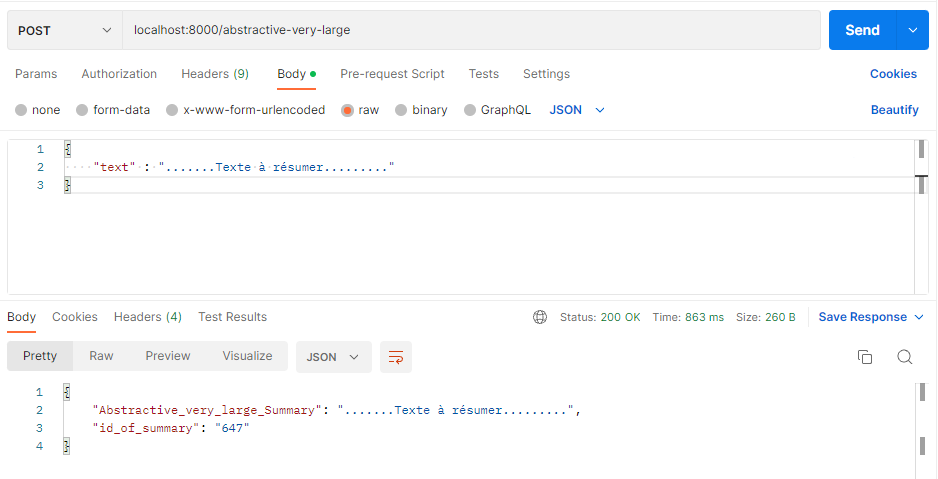
\includegraphics[width=15cm]{AbstractiveVeryLarge.PNG}
\end{center}

Pour l'\textit{end-point} \textbf{\textit{POST /abstractive-barthez}}, voici également un exemple :
\begin{center}
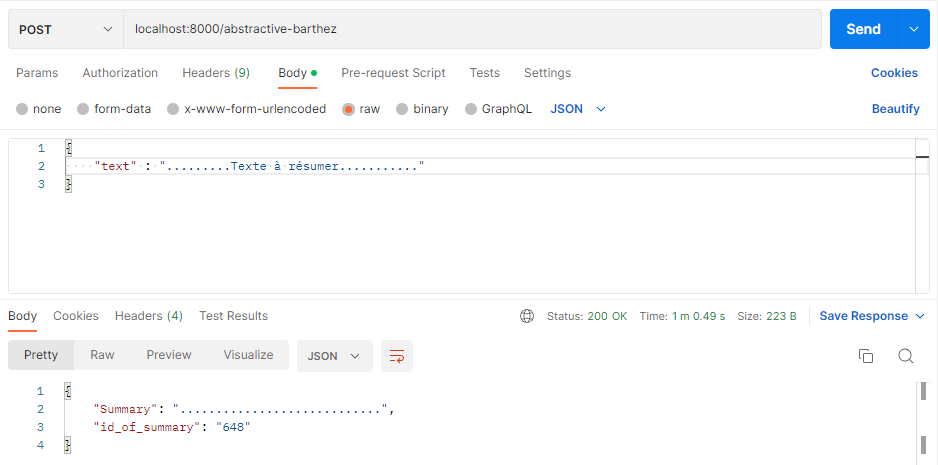
\includegraphics[width=15cm]{BARThez.PNG}
\end{center}
Pour l'\textit{end-point} \textbf{\textit{POST /abstractive-experimental-bartkrame}}, voici aussi un exemple :
\begin{center}
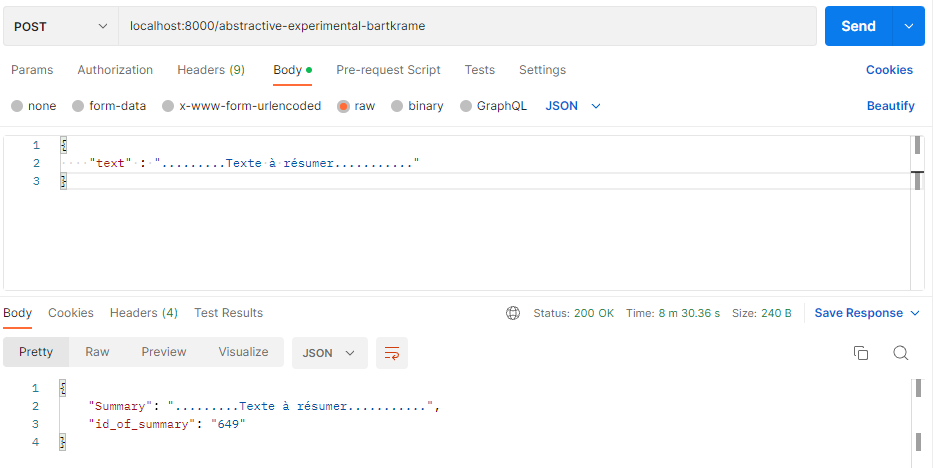
\includegraphics[width=15cm]{BARTkrame.PNG}
\end{center}

Finalement, pour l'évaluation des résumés, c'est-à-dire l'end-point \textbf{\textit{POST /evaluation}}, voici un exemple complet de requête :
\begin{itemize}
\item[•] En cas de réussite :
\begin{center}
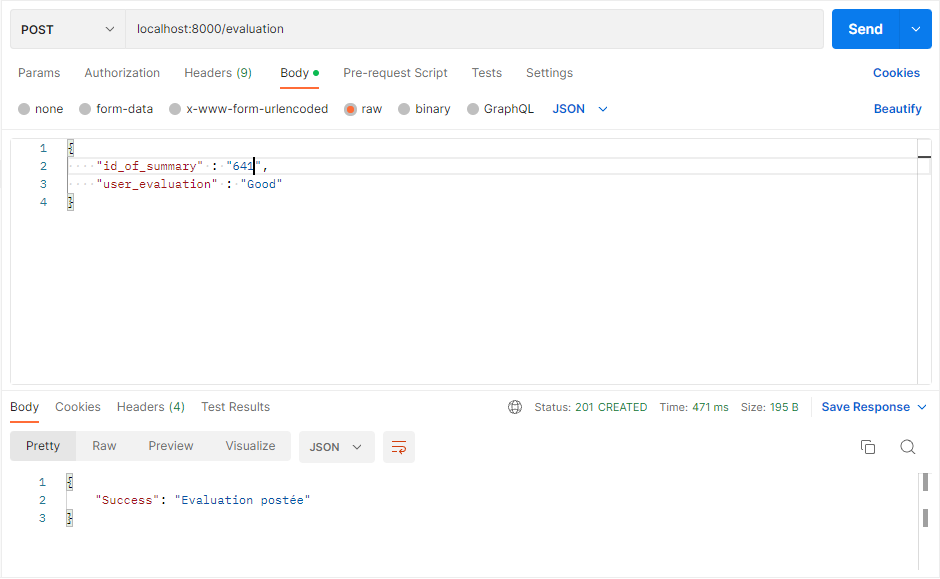
\includegraphics[width=15cm]{EvaluationSuccess.PNG}
\end{center}
\item[•] En cas d'échec :
\begin{center}
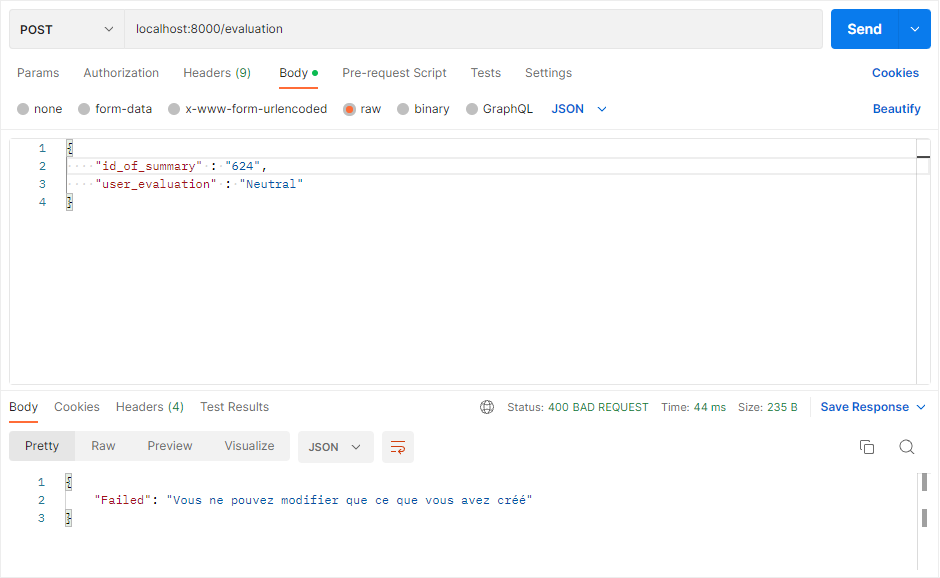
\includegraphics[width=15cm]{EvaluationFailed.PNG}
\end{center}
\end{itemize}
